% ============================================================
% Section 3: System Architecture
% ============================================================
\section{System Architecture}
\label{sec:architecture}

\subsection{Data Source}

The engine operates on the NewsFeed API. Each API response contains a list of news items, where each item includes:

\begin{itemize}
    \item \textbf{Textual fields}: \texttt{title} (headline), \texttt{source} (e.g., BBG, CNBC, FT, Reuters), \texttt{description} (extended text), \texttt{url}, \texttt{publishedAt} (ISO 8601 timestamp).
    \item \textbf{Price snapshots} (22 concurrent numeric fields at headline time): futures prices for S\&P 500 E-mini (\texttt{esf}, \texttt{pc\_esf}), Nasdaq-100 (\texttt{nqf}, \texttt{pc\_nqf}), and crude oil (\texttt{clf}, \texttt{pc\_clf}); ETF prices for SPX (\texttt{spx}, \texttt{pc\_spx}), DJIA (\texttt{djia}, \texttt{pc\_djia}), NDX (\texttt{ndx}, \texttt{pc\_ndx}), SPY (\texttt{spy}, \texttt{pc\_spy}), IWM (\texttt{iwm}, \texttt{pc\_iwm}), and DIA (\texttt{dia}, \texttt{pc\_dia}); and cryptocurrency prices for Bitcoin (\texttt{btc}, \texttt{pc\_btc}) and Ethereum (\texttt{eth}, \texttt{pc\_eth}).
\end{itemize}

The critical design insight is that each news item carries a timestamp \texttt{publishedAt} and a concurrent price level for each asset. By joining against the engine's own price time series---polled from the API's concurrent snapshots every polling cycle---the system computes the forward 24-hour price impact for each headline. This creates a natural supervised signal: the percentage change in ES futures (and each other asset) from the snapshot level to the level approximately 24 hours later.

\subsection{Pipeline Overview}

The system runs as a four-stage Hermes cron pipeline on a 3-hour cycle (configurable):

\begin{equation}
\text{Ingest} \rightarrow \text{Score} \rightarrow \text{Cluster} \rightarrow \text{Calibrate}
\label{eq:pipeline}
\end{equation}

Figure~\ref{fig:pipeline} shows the data flow.

\begin{figure}[ht]
\centering
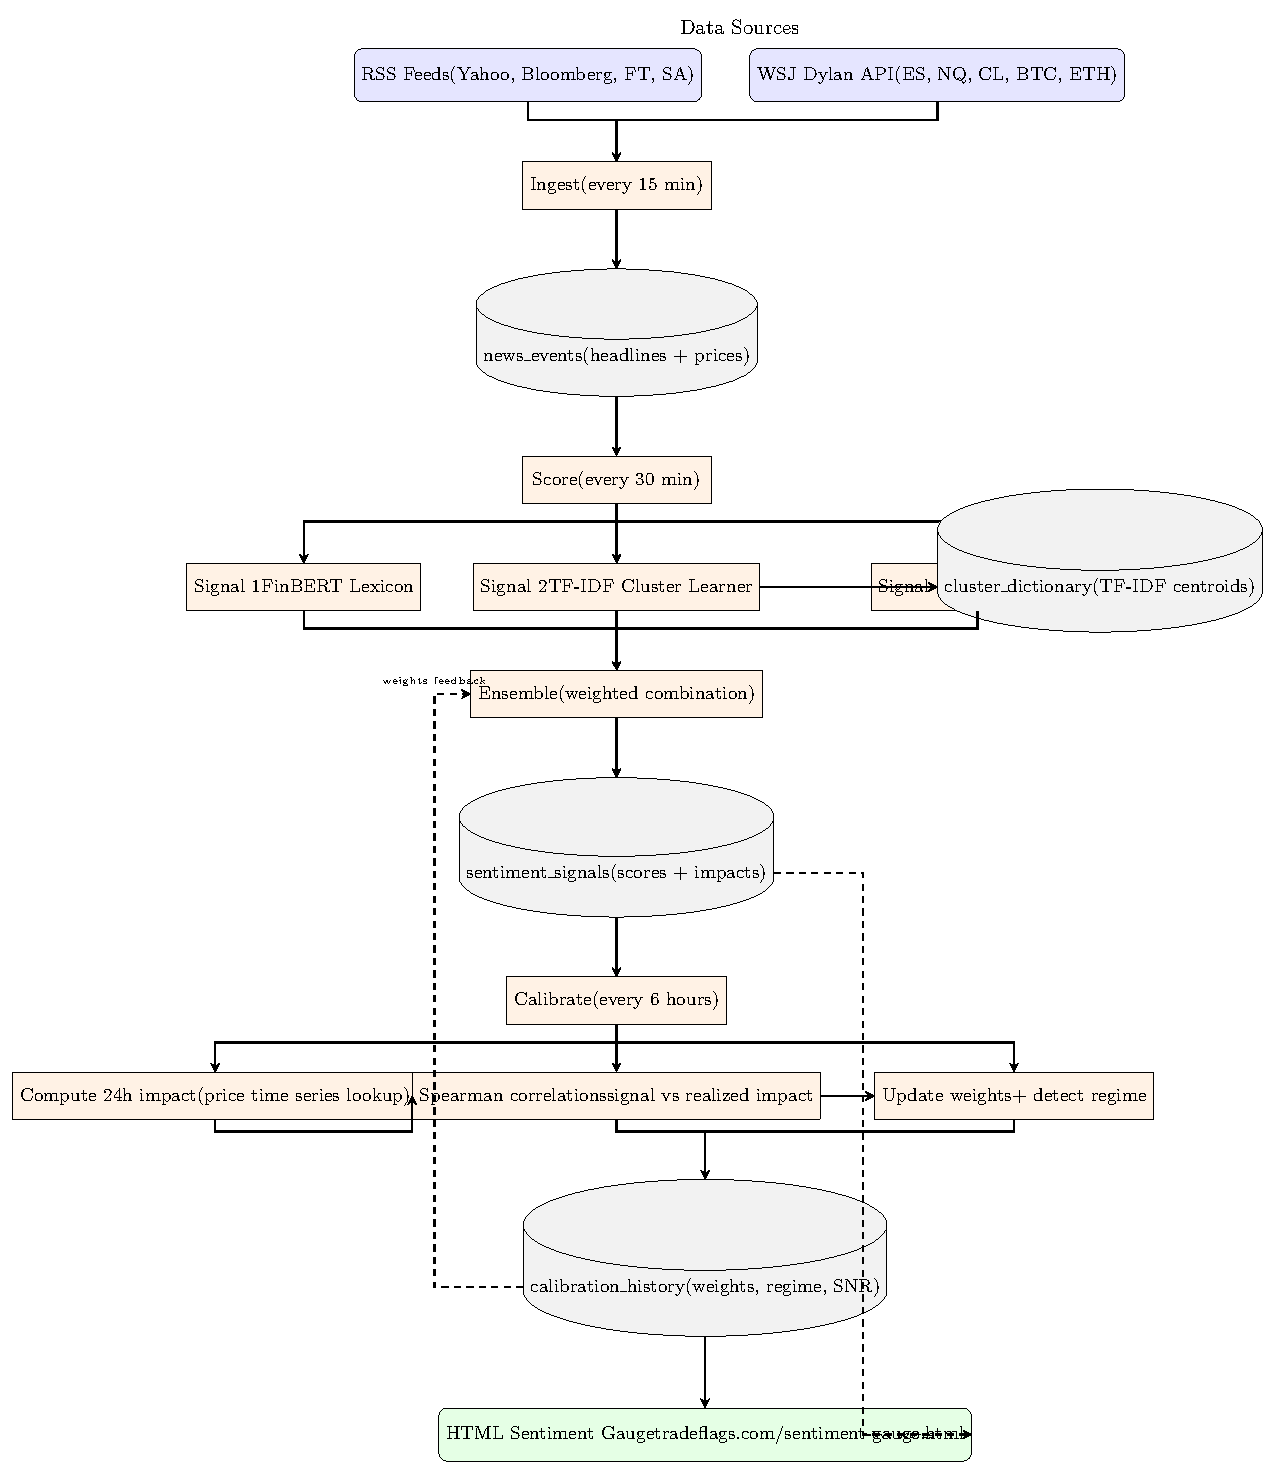
\includegraphics[width=0.95\textwidth]{figures/pipeline-flowchart.pdf}
\caption{End-to-end pipeline architecture. The API feeds into the ingest stage, which writes to \texttt{news\_events} in MySQL. The scoring stage computes three parallel sentiment signals. The cluster stage maintains the TF-IDF centroid dictionary. The calibration stage computes 24h forward price impacts, adjusts ensemble weights, and detects market regime. Dashed arrows represent the weights feedback loop.}
\label{fig:pipeline}
\end{figure}

\subsection{MySQL Schema}

The system uses four MySQL tables on a local server (\texttt{10.0.0.44:3306}, database \texttt{stocks}):

\subsubsection{\texttt{news\_events}}

Stores raw ingested news with their paired price snapshots. As of June 2026, the table contains over 430,000 headline--price pairings spanning approximately two years of market data. Each row carries a \texttt{headline\_hash} (SHA-256 of normalized headline + publication date) for exact deduplication via a \texttt{UNIQUE KEY} constraint. The table has 22 numeric columns for price data plus metadata columns (\texttt{source}, \texttt{url}, \texttt{published\_at}, \texttt{ingested\_at}).

\subsubsection{\texttt{sentiment\_signals}}

Stores computed sentiment scores for each news event. One row per news event, populated by the scoring pipeline. Contains the three individual signal scores (FinBERT lexicon, statistical cluster, LLM) with confidence metrics, plus the ensemble score. Crucially, the table stores \texttt{realized\_pc\_esf\_5min}---the actual 24-hour percentage change of ES futures following each headline, populated by lookups into the price time series---and \texttt{prediction\_error}, the difference between the ensemble score (normalized) and the realized move.

\subsubsection{\texttt{cluster\_dictionary}}

Stores the TF-IDF cluster centroids. Each row represents a semantic cluster of headlines with: centroid vector (stored as JSON), rolling average price reactions across five assets (ES, NQ, BTC, CL, ETH), sample count, keyword label, Sharpe ratio (mean/std of realized impacts), last-updated timestamp, and an active flag. Pruned regularly by the cluster maintenance job.

\subsubsection{\texttt{calibration\_history}}

Stores the rolling calibration record. Each row covers a 7-day calibration window containing: the Spearman correlation of each signal (LLM, FinBERT, statistical) against realized price moves, the optimal ensemble weights for that window, the detected market regime (bullish/bearish/neutral/volatile), and the signal-to-noise ratio ($\rho_{\text{ensemble}}^2$).

\subsubsection{\texttt{cluster\_vocab}}

A supplementary table that stores the persistent TF-IDF vocabulary (top 5,000 terms by IDF weight) as a JSON blob. This ensures vocabulary consistency across scoring cycles: the same term-to-index mapping is reused until the next cluster rebuild.

\subsection{Dual-Layer Deduplication Strategy}

The API may push the same headline across multiple polling cycles, sometimes with slightly different timestamps or minor rewording. CRANE enforces a strict two-tier isolation protocol:

\begin{enumerate}
    \item \textbf{Exact cryptographic dedup}: The \texttt{headline\_hash} is computed from the normalized headline (lowercased, stripped, punctuation-removed) plus publication date only (not timestamp). The MySQL \texttt{UNIQUE KEY} constraint silently rejects duplicates via \texttt{INSERT IGNORE}.

    \item \textbf{Fuzzy linguistic dedup}: For headlines with character trigram Jaccard similarity $\geq 0.85$ to any headline in the last 24 hours, the item is classified as a near-duplicate and skipped. This catches minor rewording, case changes, and trailing punctuation variations across API refreshes.
\end{enumerate}
